\documentclass[sigconf]{acmart}
\usepackage{amsmath}
\usepackage{booktabs}
\usepackage{graphicx}
\usepackage{longtable}
\usepackage{array}
\setlength{\emergencystretch}{1.5em}
\usepackage{float}
% The immediately following \clearpage enforces the manuscript float boundary;
% keep an explicit semantic marker without requiring the optional placeins package.
\providecommand{\FloatBarrier}{}

\settopmatter{printacmref=false}
\setcopyright{none}
\acmConference[Data Mining Course Project]{Data Mining Course Research Report}{2026}{Shanghai, China}
\acmBooktitle{Data Mining Course Research Report}
\acmDOI{}
\acmISBN{}
% Generated by scripts/57_write_final_paper.py from Phase 3 CSVs.
\newcommand{\NPeople}{661{,}124}
\newcommand{\NEntry}{220{,}627}
\newcommand{\GlobalDfiveRoc}{0.936956}
\newcommand{\GlobalDfivePr}{0.882535}
\newcommand{\GlobalDfiveLogLoss}{0.315106}
\newcommand{\GlobalDfiveBrier}{0.097356}
\newcommand{\GlobalDfiveEce}{0.003438}
\newcommand{\SourceEligible}{452,035}
\newcommand{\SourceGroups}{145}
\newcommand{\SourceLargest}{448,632}
\newcommand{\SourceLargestPct}{99.25\%}
\newcommand{\DsiFamilyShare}{2.87\%}


\makeatletter
\setlength{\@fptop}{0pt}
\setlength{\@fpsep}{12pt}
\setlength{\@fpbot}{0pt plus 1fil}
\makeatother
\renewcommand{\topfraction}{0.95}
\renewcommand{\bottomfraction}{0.95}
\renewcommand{\textfraction}{0.06}
\renewcommand{\floatpagefraction}{0.78}
\setlength{\textfloatsep}{12pt plus 3pt minus 3pt}
\setlength{\floatsep}{10pt plus 3pt minus 3pt}

\begin{document}

\title{Who Leaves a Recorded Path into Government?\\Structure, Documentation, and Distribution Shift in CBDB}
\ifanonymous
  \author{Anonymous Author(s)}
  \affiliation{\institution{Anonymous Institution}\country{}}
\else
  \author{\PaperAuthorName}
  \affiliation{\institution{\PaperInstitution}\city{Shanghai}\country{China}}
\fi

\begin{abstract}
Prosopographical databases make collective historical analysis possible, but their records reflect source survival, editorial priorities, and database encoding. We predict whether each of \NPeople{} China Biographical Database (CBDB) people has an \texttt{ENTRY\_DATA} record. This operational label, $E$, differs from both posting-record presence, $P$, and the latent state of true historical entry, $T$. We therefore estimate retrospective record presence rather than historical truth. Frozen logistic and CatBoost models were evaluated through grouped ablation, paired bootstrap, five-seed stability, family and spatial shifts, validation-fitted calibration, and grouped SHAP. The designated D5\_MAIN model reached Global ROC-AUC \GlobalDfiveRoc{} and PR-AUC \GlobalDfivePr{}. Conditional evidence was strongest for gender, address observability, administrative geography, and family observability, whereas recorded family political capital added little after observability and topology. Discrimination weakened on matched-support unseen historical regions. Full-coverage source-group confirmation was infeasible under the prespecified connected-component protocol because 448,632 of 452,035 eligible people belonged to a single connected component. These results show that CBDB ENTRY-record presence is highly predictable, while also locating that performance within the database's documentation and selection processes. They do not reconstruct true historical entry or identify causal effects.
\end{abstract}

\ccsdesc[500]{Computing methodologies~Supervised learning by classification}
\ccsdesc[300]{Applied computing~Digital libraries and archives}
\keywords{computational history, prosopography, documentation bias, distribution shift, CBDB}

\maketitle
\ifanonymous
  \hypersetup{pdftitle={Who Leaves a Recorded Path into Government? Structure, Documentation, and Distribution Shift in CBDB},pdfauthor={Anonymous Author(s)}}
\else
  \hypersetup{pdftitle={Who Leaves a Recorded Path into Government? Structure, Documentation, and Distribution Shift in CBDB},pdfauthor={\PaperAuthorName}}
\fi

\section{Introduction}
Prosopographical databases convert dispersed biographical traces into relational data for collective, spatial, and network analysis \cite{bol2012gis,fullerwang2021networks,chenwang2022cbdb}. CBDB is a prominent example, combining structured biographies with relations, places, offices, kinship, and texts \cite{cbdb2026,fuller2024,tsui2020harvesting}. Such databases are not random censuses of past populations. Their contents depend on which people entered surviving sources, which sources were processed, and how ambiguous statements were encoded.

This study combines open-ended exploratory analysis of dynastic, gender, ENTRY-pathway, geographic, and kin-observability patterns with predictive modeling of ENTRY-record presence.

This selection creates a specific prediction problem. ENTRY-record presence may reflect historical structure, including period, geography, and family relations. It may also reflect the documentation process that made those attributes and the label observable. Consequently, a high area under the receiver-operating-characteristic curve (ROC-AUC) is insufficient evidence of historical recovery. The central problem is to separate predictive structure from record-generation signals and to state where that separation fails.

We ask five questions. \textbf{RQ1} asks whether ENTRY-record presence can be predicted reliably on a frozen person-level test. \textbf{RQ2} asks how personal, geographic, family, and documentation blocks contribute conditionally. \textbf{RQ3} asks whether recorded family political capital adds information after observability and topology. \textbf{RQ4} asks how the frozen F2 structural comparator changes under whole-family grouping and how locked models transport to unseen historical regions. \textbf{RQ5} asks how far high performance reflects historical structure versus database recording processes.

The study contributes a reproducible measurement and leakage policy, a frozen three-level model hierarchy, and an evidence-ordered interpretation. H\_STRUCT is a historical structural benchmark, although it still contains address and kin observability. D5\_MAIN is the designated predictive model without relatives' outcomes. D6\_UPPER is a database-internal record-structure upper bound. Grouped ablation and distribution shifts carry the main interpretation; SHAP is retained only as subordinate attribution evidence.

\section{Related Work}
\textbf{Computational prosopography.} CBDB supports statistical, network, spatial, kinship, and reference analysis of heterogeneous historical texts \cite{tsui2020harvesting,chenwang2022cbdb,fullerwang2021networks,bol2012gis}. Its official guide documents schema and export procedures, not complete historical coverage \cite{fuller2024}.

\textbf{Prediction and generalization.} Tree ensembles are strong heterogeneous-tabular baselines, and CatBoost limits target leakage in categorical statistics \cite{grinsztajn2022tabular,prokhorenkova2018catboost}. Random holdout can be optimistic under structured dependence, while covariate shift can invalidate ordinary validation \cite{roberts2017cv,sugiyama2007covariate}. WILDS and transport research motivate explicitly bounded shift tests \cite{koh2021wilds,subbaswamy2019transport}.

\textbf{Measurement, attribution, and calibration.} Administrative data inherit selection processes; operational measures need not equal latent constructs, and imperfect labels alter classification evidence \cite{hand2018administrative,jacobs2021measurement,frenay2014label}. Dataset documentation should expose these boundaries \cite{gebru2021datasheets}. SHAP is neither context-free importance nor causal evidence, and calibration requires held-out fitting data \cite{lundberg2017shap,kumar2020shap,niculescu2005probabilities,guo2017calibration}.

\section{Data and Measurement Problem}
The frozen input is official release \texttt{cbdb\_20260829.sqlite3}. The assignment brief reports approximately 515,488 people, whereas the verified release used in this study contains 661,124 \texttt{BIOG\_MAIN} person records. CBDB counts are release-specific; all results here refer only to \texttt{cbdb\_20260829.sqlite3}. CBDB is a selectively assembled historical database rather than a population register. Relation tables were aggregated by person before joining to \texttt{BIOG\_MAIN}, which prevented multi-table fan-out. The resulting analysis population contains \NPeople{} covered people and \NEntry{} positive ENTRY labels (Table~\ref{tab:dataset}).

\texttt{ENTRY\_DATA} includes examination or degree records, school or student status, recommendation, hereditary or \emph{yin} privilege, military entry, purchase or donation, direct appointment, and other or ambiguous entry records. Define $E_i=1$ when person $i$ has at least one ENTRY row and $P_i=1$ when the person has at least one valid posting row. Let $T$ denote the latent true historical state of entry into government. At the construct level,
\begin{equation}
E \not\equiv T,\qquad P \not\equiv T,\qquad E \not\equiv P.
\end{equation}
E, P, and T are distinct constructs and are not semantically equivalent. Thus $E=0$ means that no ENTRY row was found, while $E=1$ does not necessarily imply actual office holding. Posting is also incomplete and cannot serve as historical ground truth. The estimand is $\Pr(E_i=1\mid X_i)$.

\begin{figure*}[t]
\centering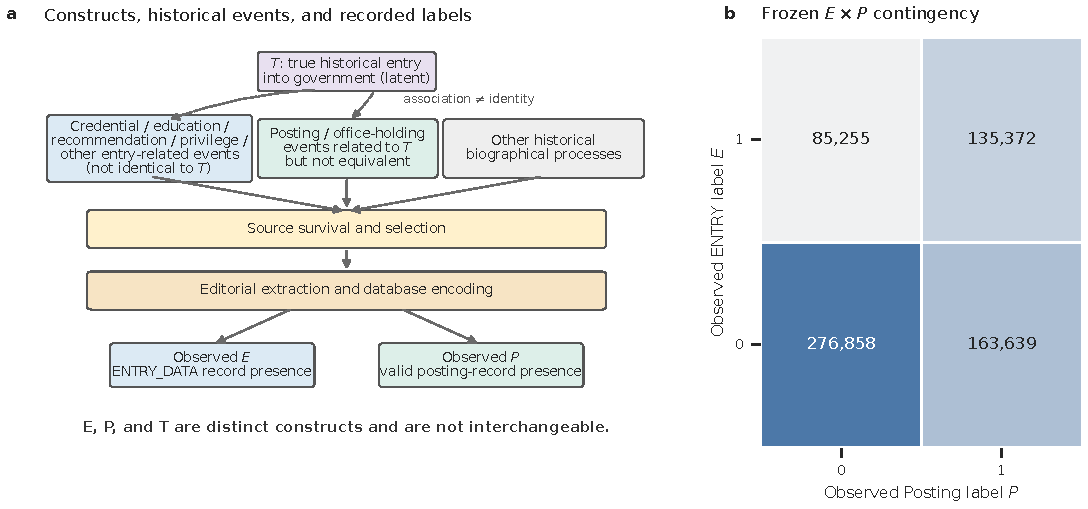
\includegraphics[width=0.94\textwidth]{figures/final_task_definition_ep_t.pdf}
\caption{\textbf{Constructs, historical events, and recorded labels.} \textbf{a}, $T$ is latent true historical entry. Credential, education, recommendation, privilege, and other entry-related events are not $T$; posting or office-holding events are related to, but not equivalent to, $T$. Source survival, extraction, and encoding produce the observed $E$ and $P$ relations. $E$, $P$, and $T$ are distinct constructs and are not interchangeable. \textbf{b}, Frozen contingency for all \NPeople{} CBDB-covered people.}
\Description{A process diagram separates entry, posting, and other biographical events before source selection and encoding. A two-by-two matrix gives frozen counts for observed ENTRY and posting labels.}
\label{fig:ept}
\end{figure*}
\begin{table*}[t]
\caption{Dataset and observed targets. Counts and shares are generated from the frozen person target and E--P contingency tables.}
\label{tab:dataset}
\centering
\begin{tabular}{lrl}
\toprule
Quantity & Value & Operational definition \\
\midrule
CBDB-covered people & 661,124 & One row per BIOG\_MAIN person \\
E positives & 220,627 & At least one ENTRY\_DATA row \\
E prevalence & 0.3337 & Recorded ENTRY share among CBDB-covered people \\
P positives & 299,011 & At least one valid posting record \\
Primary-test people & 99,307 & Frozen dynasty-by-E stratified test \\
\bottomrule
\end{tabular}
\end{table*}


Figure~\ref{fig:ept}b makes the proxy boundary concrete. The $E=1,P=1$ quadrant records both an ENTRY and a posting trace. The $E=1,P=0$ quadrant records ENTRY without a valid posting, while $E=0,P=1$ records posting without ENTRY. The $E=0,P=0$ quadrant records neither relation. None of these quadrants identifies $T$ without additional historical evidence.

\section{Task Definition and Leakage Control}
The primary task classifies retrospective ENTRY-record presence. Direct ENTRY fields, the focal person's posting outcomes, entry or posting counts, raw index year, and person or family identifiers are forbidden predictors. Safe birth information requires audited provenance. Regional density is fitted on training people only. The local ENTRY prior groups the exact \texttt{addr\_id} key, applies five-fold deterministic out-of-fold encoding with smoothing strength 20 on training people, and transforms validation or test people from the complete-training mapping; unseen keys use the relevant training mean. Test labels select neither features nor hyperparameters, thresholds, early stopping, or calibration.

The model hierarchy isolates progressively more database structure (Table~\ref{tab:features}). H\_STRUCT contains regime, gender, safe birth cohort, geography, address availability, and kin observability or topology. It is therefore not an unbiased historical model. D5\_MAIN adds documentation-linked features and a supervised local prior but excludes relatives' outcomes. D6\_UPPER adds full-record relatives' lifetime ENTRY and posting summaries. Those temporally ambiguous fields make D6\_UPPER an upper bound rather than a historical mechanism model.
\begin{table*}[t]
\caption{Locked model roles and leakage boundary. Feature counts are read from the Phase 2.6 lock artifact.}
\label{tab:features}
\centering
\resizebox{\textwidth}{!}{%
\begin{tabular}{lrll}
\toprule
Model & Features & Role & Boundary \\
\midrule
\texttt{H\_STRUCT} & 26 & Historical structural benchmark & No general documentation, address type, local target prior, or relative outcomes \\
\texttt{D5\_MAIN} & 34 & Main predictive model & Documentation and topology; no relative outcomes \\
\texttt{D6\_UPPER} & 44 & Record-structure upper bound & D5 plus full-record relative ENTRY/posting outcomes \\
\bottomrule
\end{tabular}}
\end{table*}


\section{Exploratory Data Analysis}
Across Tang, Song, Yuan, Ming, and Qing, CBDB coverage ranged from 25,310 to 237,423 people and $E$ prevalence from 3.17\% to 54.54\% (Figure~\ref{fig:dynasty}). Historical institutions, corpus composition, database projects, and source survival remain inseparable explanations.

\begin{figure*}[t]
\centering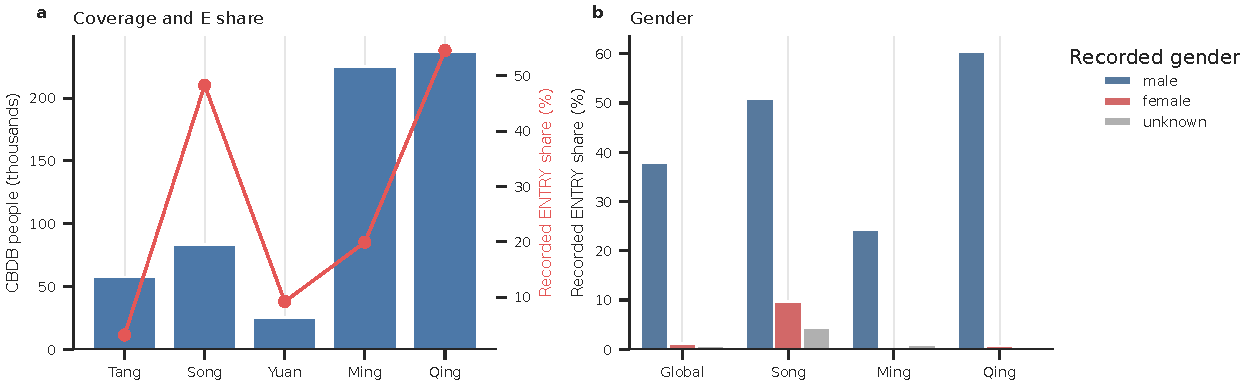
\includegraphics[width=0.92\textwidth]{figures/fig2_dynasty_gender.pdf}
\caption{\textbf{CBDB coverage and recorded ENTRY share.} \textbf{a}, Covered people and $E$ prevalence within Tang, Song, Yuan, Ming, and Qing. \textbf{b}, $E$ prevalence within recorded gender groups for Global, Song, Ming, and Qing. Denominators are CBDB-covered people, not historical populations.}
\Description{Bars show CBDB-covered people and recorded ENTRY shares by dynasty and gender.}
\label{fig:dynasty}
\end{figure*}

Recorded gender is also imbalanced: 87.55\% of covered people are male, and $E$ prevalence is 37.96\% for men, 1.22\% for women, and 0.79\% for unknown gender. This predictive partition is not a historical comparison of opportunity.

ENTRY pathways vary across dynasties (Figure~\ref{fig:pathways}). Examination, schooling, recommendation, privilege, military, and appointment categories are nonexclusive at person level. Their heterogeneity may reflect historical access, terminology, or source processing.

\begin{figure*}[t]
\centering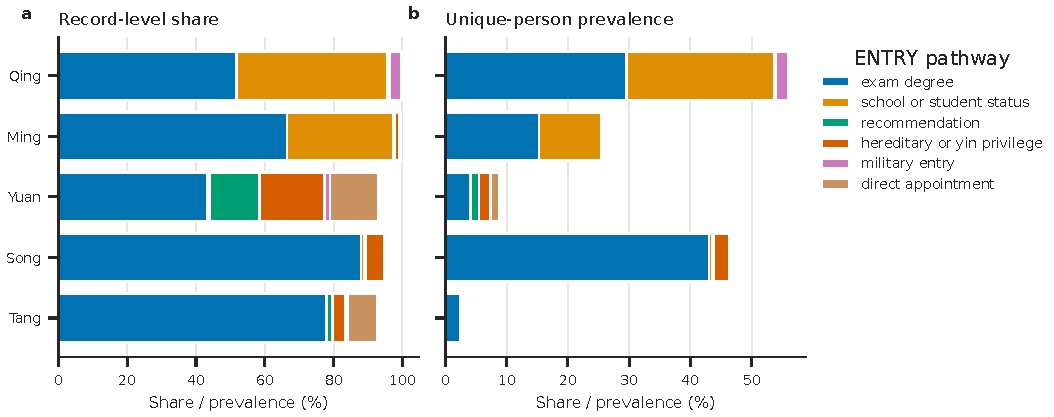
\includegraphics[width=0.92\textwidth]{figures/fig3_entry_pathways.pdf}
\caption{\textbf{Recorded ENTRY pathway composition.} \textbf{a}, Share of ENTRY records by semantic category and dynasty. \textbf{b}, Prevalence of each category among all CBDB-covered people in that dynasty. Person-level pathways are nonexclusive and may sum above 100\%.}
\Description{Stacked horizontal bars compare record-level and person-level ENTRY pathway shares for five dynasties.}
\label{fig:pathways}
\end{figure*}

Observability differs by feature: addresses cover 59.83\% of people, any kin 43.29\%, core family 33.94\%, valid coordinates 57.82\%, and safe birth years 9.05\%. Documentation intensity also varies by population, allowing models to learn record production alongside historical attributes.

\section{Feature Construction}
Features separate personal attributes; address observability, administrative and physical geography, density, semantics, and local prior; family observability, topology, and capital; and general documentation flags.

Administrative identifiers mix place and normalization; address and kin flags directly measure observability; family topology is partly transductive; and relatives' outcomes are not strictly pre-entry. Grouped ablations preserve these boundaries.

\section{Models and Evaluation Protocol}
Balanced logistic regression is the frozen linear baseline. CatBoost models use seed 42, at most 500 iterations, depth 7, learning rate 0.05, $L_2$ leaf regularization 5, and validation-only early stopping. No Phase 3.1 model was trained or tuned. The primary split is a frozen, person-level, dynasty-by-$E$ stratification. Whole-family robustness keeps connected family groups disjoint. Matched-support spatial tests compare random and unseen-region tests within the same reliable-prefecture support, although their test people differ.

We report ROC-AUC, precision-recall AUC (PR-AUC), balanced accuracy, F1, log loss, Brier score, and expected calibration error (ECE). PR-AUC is interpreted with test prevalence. The sigmoid calibrator was fitted on validation predictions only. Table~\ref{tab:performance} labels raw log loss and Brier score separately from validation-calibrated ECE. Paired bootstrap used 500 stratified resamples only when the exact prediction pair was retained. These intervals quantify test-sample variability, not uncertainty in label validity, source survival, or inclusion in CBDB.

Five prespecified seeds assess stability for selected contrasts. The SAFE temporal split is reported as a split diagnostic because no frozen locked-model performance artifact exists. Qing is descriptive because no prespecified Qing holdout was frozen. A source-group model was conditional on a feasibility gate and was not fitted because full-coverage confirmation was infeasible under the prespecified full-coverage connected-component protocol.

\section{Experimental Results}
\subsection{Locked models establish strong within-database discrimination}
Table~\ref{tab:performance} and Figure~\ref{fig:models} establish the frozen hierarchy. Global D5\_MAIN achieved ROC-AUC \GlobalDfiveRoc{} and PR-AUC \GlobalDfivePr{}, with raw log loss \GlobalDfiveLogLoss{} and raw Brier score \GlobalDfiveBrier{}. Its validation-calibrated ECE was \GlobalDfiveEce{}. Performance also remained high in Song and Ming, although population prevalence and PR-AUC differed.

D6\_UPPER improved only marginally over D5\_MAIN. Because it includes relatives' lifetime ENTRY and posting information, the comparison bounds record-structure predictability rather than supporting a stronger historical interpretation. H\_STRUCT performed below D5\_MAIN but remained strong, showing that regime, geography, family structure, and their observability already contain substantial predictive signal.
\begin{table*}[t]
\caption{Frozen primary-test performance. Log loss and Brier score use raw model probabilities; ECE uses probabilities from a sigmoid calibrator fitted on validation predictions only. The logistic artifact did not retain a directly comparable calibrated ECE. D5\_MAIN is the designated main result.}
\label{tab:performance}
\centering
\begin{tabular}{llrrrrr}
\toprule
Population & Model & ROC-AUC & PR-AUC & Raw LogLoss & Raw Brier & Validation-calibrated ECE \\
\midrule
Global & Logistic M6 & 0.9160 & 0.8436 & 0.3635 & 0.1128 & -- \\
Global & H\_STRUCT & 0.9267 & 0.8582 & 0.3393 & 0.1048 & 0.0036 \\
Global & \textbf{D5\_MAIN} & 0.9370 & 0.8825 & 0.3151 & 0.0974 & 0.0034 \\
Global & D6\_UPPER & 0.9374 & 0.8831 & 0.3140 & 0.0969 & 0.0034 \\
Song & Logistic M6 & 0.9008 & 0.8810 & 0.3985 & 0.1223 & -- \\
Song & H\_STRUCT & 0.9183 & 0.9116 & 0.3604 & 0.1112 & 0.0072 \\
Song & \textbf{D5\_MAIN} & 0.9384 & 0.9398 & 0.3089 & 0.0940 & 0.0094 \\
Song & D6\_UPPER & 0.9398 & 0.9412 & 0.3055 & 0.0928 & 0.0102 \\
Ming & Logistic M6 & 0.9021 & 0.7765 & 0.3500 & 0.1126 & -- \\
Ming & H\_STRUCT & 0.9107 & 0.7799 & 0.3463 & 0.1097 & 0.0029 \\
Ming & \textbf{D5\_MAIN} & 0.9164 & 0.8005 & 0.3229 & 0.1026 & 0.0027 \\
Ming & D6\_UPPER & 0.9167 & 0.8012 & 0.3224 & 0.1023 & 0.0025 \\
\bottomrule
\end{tabular}
\end{table*}


\begin{figure*}[t]
\centering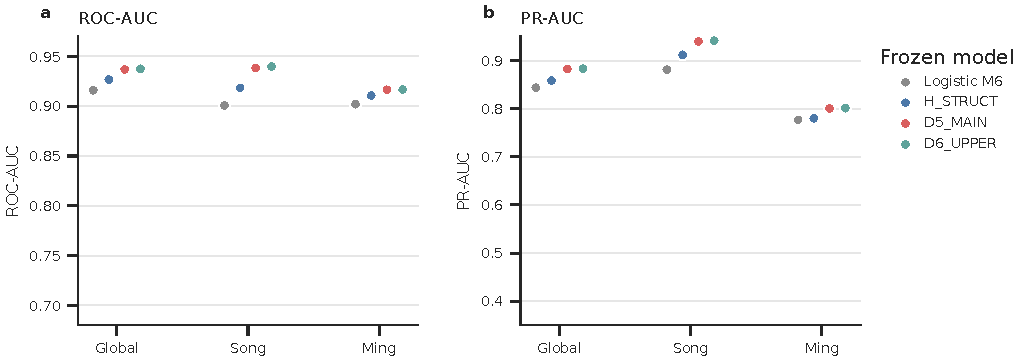
\includegraphics[width=0.92\textwidth]{figures/fig4_locked_models.pdf}
\caption{\textbf{Frozen primary-test discrimination.} ROC-AUC and PR-AUC compare the logistic baseline, H\_STRUCT, D5\_MAIN, and D6\_UPPER in Global, Song, and Ming. D5\_MAIN is the designated main model; D6\_UPPER is a database-internal upper bound.}
\Description{Two point plots compare ROC-AUC and PR-AUC across populations and frozen models.}
\label{fig:models}
\end{figure*}

\subsection{Ablation separates observability from family capital}
Grouped ablation is the primary evidence of conditional information (Figure~\ref{fig:ablation}; Table~\ref{tab:ablation}). Global increments were largest for gender, address observability, administrative geography, and family observability. Address-record semantics added a smaller but visible increment. Physical geography changed ROC-AUC by 0.000014 and PR-AUC by $-0.000343$. Its exact A2/A3 paired predictions were not retained, so no valid confidence interval is reported. Because the grouped ablations follow a prespecified nested order, every increment is conditional on the blocks already entered. The increments are therefore order-dependent and cannot be interpreted as unique contributions or causal effects.

Family observability increased Global ROC-AUC by 0.0217, while topology added 0.0023 (95\% paired bootstrap interval 0.0019 to 0.0026). Full-record family capital added 0.0007 (0.0005 to 0.0009), and train-observed capital added 0.0003 (0.0001 to 0.0005). These positive increments are stable but substantively small after observability and topology. Five-seed ranges in Appendix Figure~\ref{fig:multiseed} support the same ordering.

\begin{figure*}[t]
\centering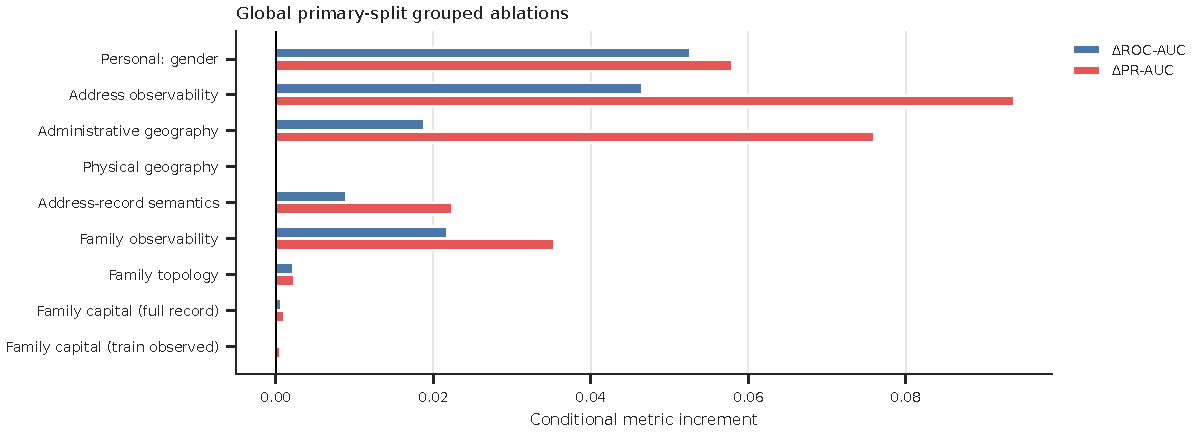
\includegraphics[width=0.92\textwidth]{figures/fig5_grouped_ablation.pdf}
\caption{\textbf{Global grouped ablations.} Bars show conditional ROC-AUC and PR-AUC changes for prespecified nested feature blocks. Negative values extend left of zero. Unsupported intervals are omitted because exact paired predictions were not retained for every contrast.}
\Description{Horizontal paired bars show conditional metric increments for nine feature blocks.}
\label{fig:ablation}
\end{figure*}
\begin{table*}[t]
\caption{Global grouped ablation evidence. Point estimates are frozen conditional increments. Intervals are 500-resample paired bootstrap intervals only where the exact paired prediction pair was retained. Dashes, including Physical Geography, mean that no valid exact-pair interval is available, not zero uncertainty.}
\label{tab:ablation}
\centering
\begin{tabular}{lrrrr}
\toprule
Feature block & $\Delta$ROC & 95\% CI & $\Delta$PR & 95\% CI \\
\midrule
Personal: gender & +0.0526 & -- & +0.0580 & -- \\
Address observability & +0.0465 & -- & +0.0939 & -- \\
Administrative geography & +0.0188 & -- & +0.0761 & -- \\
Physical geography & +0.0000 & -- & -0.0003 & -- \\
Address-record semantics & +0.0090 & -- & +0.0224 & -- \\
Family observability & +0.0217 & -- & +0.0354 & -- \\
Family topology & +0.0023 & [0.0019, 0.0026] & +0.0024 & [0.0018, 0.0029] \\
Family capital (full record) & +0.0007 & [0.0005, 0.0009] & +0.0011 & [0.0007, 0.0015] \\
Family capital (train observed) & +0.0003 & [0.0001, 0.0005] & +0.0005 & [0.0002, 0.0009] \\
\bottomrule
\end{tabular}
\end{table*}


\subsection{Family and spatial shifts bound generalization}
Address decomposition separates a large observability increment from administrative geography, address semantics, and near-zero physical or local-prior increments (Figure~\ref{fig:spatial}a). This ordering shows conditional predictive information, not geographic causation. The matched-support test then provides a distinct boundary: unseen-region ROC-AUC decreased for H\_STRUCT and D5\_MAIN in Global, Song, and Ming (Figure~\ref{fig:spatial}b). Global decreases were 0.0307 and 0.0222, respectively.

\begin{figure*}[t]
\centering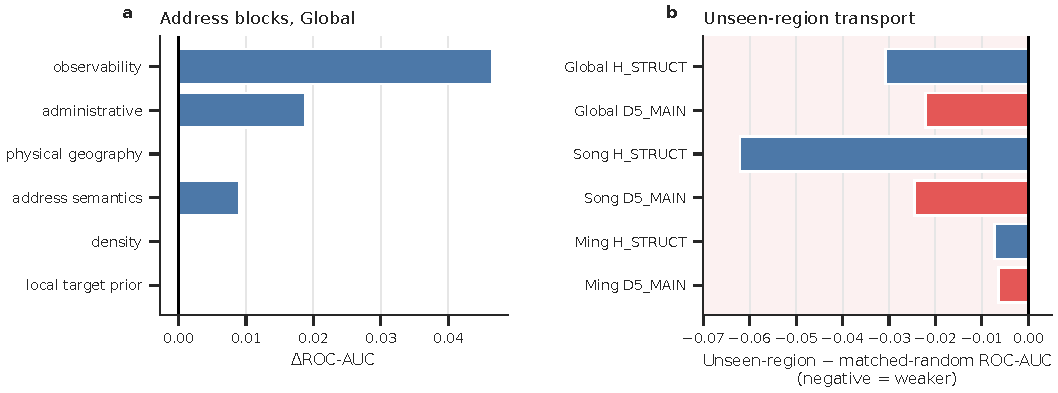
\includegraphics[width=0.92\textwidth]{figures/fig6_spatial_transport.pdf}
\caption{\textbf{Address decomposition and matched-support spatial transport.} \textbf{a}, Global conditional address-block ROC-AUC increments. \textbf{b}, Unseen-region minus matched-random ROC-AUC within reliable-prefecture support. Negative values show weaker transport, not causal geographic effects.}
\Description{Two horizontal bar plots show address-block increments and negative spatial transport deltas.}
\label{fig:spatial}
\end{figure*}

Whole-family robustness was evaluated only for the frozen F2 structural comparator in Global and Ming. Family-group robustness of D5\_MAIN was not directly evaluated. Globally and in Song, family-capital increments were small and mostly positive. The full-record F3--F2 ROC-AUC increment was +0.000701 globally and +0.001821 in Song. In Ming, the full-record increment was -0.000319 (95\% CI [-0.0009, 0.0002]) and the train-observed F4--F2 increment was -0.000394 (95\% CI [-0.0010, 0.0002]); the corresponding Ming PR-AUC intervals also included zero. Across populations, family observability and topology contributed much more predictive information than family-capital summaries (Figure~\ref{fig:family}).

\begin{figure*}[t]
\centering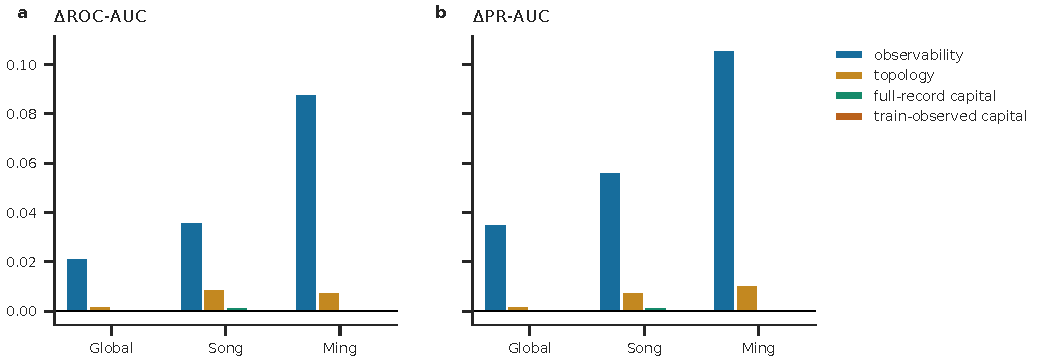
\includegraphics[width=0.92\textwidth]{figures/fig7_family_decomposition.pdf}
\caption{\textbf{Family-feature decomposition.} Conditional ROC-AUC and PR-AUC increments are shown for Global, Song, and Ming. Observability and topology are separated from full-record and train-observed political-capital summaries.}
\Description{Grouped bars compare four family feature blocks across three populations and two metrics.}
\label{fig:family}
\end{figure*}

The source audit used marked-primary person-to-source edges without the target. The largest connected component contained \SourceLargest{} of \SourceEligible{} eligible people (\SourceLargestPct{}), exceeding the prespecified 20\% ceiling. Full-coverage source-group confirmation was infeasible under the prespecified full-coverage connected-component protocol. This protocol result does not rule out a narrower source-specific validation design. A selective single-primary-source subset could support a narrower source-holdout sensitivity, but it would not represent the full CBDB-covered population.
\begin{table*}[t]
\caption{Distribution-shift evidence and its availability. Whole-family rows apply only to the frozen F2 structural comparator in Global and Ming; missing performance is labeled explicitly.}
\label{tab:robustness}
\centering
\resizebox{\textwidth}{!}{%
\begin{tabular}{lllrrl}
\toprule
Protocol & Population & Model & Shift ROC & $\Delta$ROC & Status \\
\midrule
Matched-support spatial & Global & D5\_MAIN & 0.8976 & -0.0222 & RUN \\
Matched-support spatial & Global & H\_STRUCT & 0.8724 & -0.0307 & RUN \\
Family-group holdout & Global & F2 structural comparator & 0.9272 & -0.0022 & RUN \\
Family-group holdout & Ming & F2 structural comparator & 0.9090 & -0.0032 & RUN \\
SAFE temporal & Global & Locked models & -- & -- & SPLIT\_ONLY\_NO\_LOCKED\_PERFORMANCE \\
Qing dynasty holdout & Qing & Locked models & -- & -- & NOT\_RUN\_NO\_FROZEN\_HOLDOUT \\
Source group & Global & H\_STRUCT/D5\_MAIN & -- & -- & SOURCE\_GROUP\_CONFIRMATION\_NOT\_FEASIBLE \\
\bottomrule
\end{tabular}}
\end{table*}


\section{Model Interpretation}
Grouped SHAP passed additivity checks for all nine population-model pairs (Figure~\ref{fig:shap}). Attribution shifted across populations; renaming \texttt{other} to \texttt{historical\_regime} changed only the display aggregation.

Song's local prior receives substantial SHAP share despite a near-zero conditional increment, and D6\_UPPER assigns \DsiFamilyShare{} of Global attribution to family capital despite its small increment. Correlated predictors can redistribute attribution, so SHAP is neither independent contribution nor causal effect \cite{lundberg2017shap,kumar2020shap}.

% canonical SHAP group: historical_regime
\begin{figure*}[t]
\centering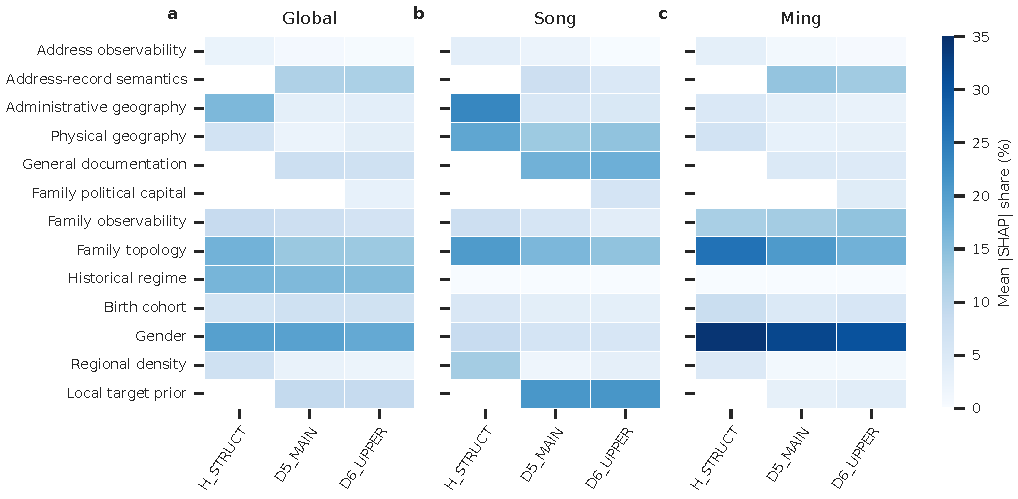
\includegraphics[width=0.92\textwidth]{figures/fig8_grouped_shap.pdf}
\caption{\textbf{Grouped mean absolute SHAP shares.} Global, Song, and Ming panels compare H\_STRUCT, D5\_MAIN, and D6\_UPPER. Physical geography comprises latitude, longitude, and distance to the dynasty-specific capital. Blank cells denote groups absent from a model. Shares are fitted-model attributions, not conditional gains or causal effects.}
\Description{Three aligned heatmaps compare grouped mean absolute SHAP shares across populations and models.}
\label{fig:shap}
\end{figure*}

\section{Discussion}
The results establish strong within-database prediction while exposing its documentary basis. H\_STRUCT retains observable geography and kin structure, D5\_MAIN gains from additional documentation-linked signals, and D6\_UPPER adds little discrimination from relatives' lifetime records.

The contribution is an auditable separation of label semantics, structural and documentation-linked increments, family-capital increments, and shift boundaries \cite{hand2018administrative,jacobs2021measurement}. Spatial degradation limits random-holdout transport, while whole-family evidence supports only F2 in Global and Ming, not D5\_MAIN.

Gender, regime, and family signals may reflect historical stratification, textual survival, editorial selection, encoding, or their combination. Source-specific or temporally anchored designs are needed to distinguish these explanations.

\section{Limitations}
\paragraph{Measurement and label validity.}
$E$ measures heterogeneous ENTRY-record presence, not $T$; $P$ is also incomplete. Bootstrap intervals cover test-sample variation for $E$, not its definition or historical validity.

\paragraph{Selection and documentation bias.}
CBDB selection varies across period, region, gender, relations, and documentation. Because these processes affect predictors and $E$, discrimination is neither population prevalence nor historical mechanism. Source confirmation was infeasible under the prespecified full-coverage connected-component protocol.

\paragraph{Temporal and transductive information.}
D5\_MAIN is retrospective, and 9.05\% safe-birth coverage prevents broad pre-entry anchoring. Family topology is partly transductive and relatives' lifetime outcomes are temporally ambiguous, restricting D6\_UPPER and family capital to database-internal bounds.

\paragraph{Generalization and adaptive test use.}
Spatial shift weakened performance, while temporal, Qing, and source-group locked performance is unavailable. Whole-family performance applies only to F2 in Global and Ming, not D5\_MAIN. Repeated project-phase test viewing creates adaptation risk; SHAP remains non-causal.

\section{Conclusion}
CBDB ENTRY-record presence is highly predictable within the frozen database. Observability and topology dominate small, Ming-uncertain family-capital increments, and unseen-region transport is weaker. Whole-family evidence is F2-only. These results concern structured records, not true entry or causal office access.

\section{Reproducibility and Availability}
\subsection{Data Availability}
This study reuses third-party CBDB data from the official release channel \cite{cbdb2026,fuller2024}. The brief reports about 515,488 people; the verified \texttt{cbdb\_20260829.sqlite3} release contains 661,124 \texttt{BIOG\_MAIN} records. Counts are release-specific, and all results use that release. Its SHA256 is verified. SQLite files are not redistributed; the package provides predictions, tables, figure sources, and regeneration code under CBDB access terms.

\subsection{Code Availability}
The package contains verification, preprocessing, frozen splits, features, evaluation, figures, environments, and tests. Its MIT License grants no CBDB redistribution rights, and no repository identifier is claimed.

\subsection{Reproducibility Statement}
Seed 42 and person splits are frozen; test labels selected neither hyperparameters nor calibration. Versions, parameters, hashes, and corrections are recorded. Run \texttt{bash} \path{scripts/run_phase3_1_1_final_polish.sh}.

\FloatBarrier
\clearpage
\label{mainend}
\bibliographystyle{ACM-Reference-Format}
\bibliography{references_final}

\clearpage
\label{appendixstart}
\appendix
\onecolumn
\setcounter{figure}{0}
\setcounter{table}{0}
\renewcommand{\thefigure}{A\arabic{figure}}
\renewcommand{\thetable}{A\arabic{table}}

\section{Target Taxonomy and Feature Boundaries}
The person-level grain begins with \texttt{BIOG\_MAIN}. ENTRY and posting relations define $E$ and $P$, while address, kin, association, status, text, institution, and source relations are aggregated separately before joining. The audited ENTRY taxonomy includes examination or degree, school or student status, recommendation, hereditary or \emph{yin} privilege, military entry, purchase or donation, direct appointment, other clear entry, failed entry, and ambiguous records. A person may occupy several categories.

The global leakage policy forbids identifiers, target fields, ENTRY or posting counts, focal posting presence, raw index-year fields, and unsafe years. Regional density is training-only, and the supervised local prior is out-of-fold on training people. F3 uses full-record relatives' outcomes; F4 restricts outcomes to training-observed relatives but is not strictly pre-entry.


\section{Exact Local Target-Prior Construction}
For population-specific training data, let \(r_i\) be the exact \texttt{addr\_id} key for person \(i\); missing keys are mapped to the literal group \texttt{\_\_MISSING\_\_}. With smoothing strength \(\alpha=20\), regional target sum \(s_r\), regional count \(n_r\), and fitting-sample target mean \(\mu\), the encoder is
\begin{equation}
\widehat p_r=\frac{s_r+\alpha\mu}{n_r+\alpha}.
\end{equation}
Training values use five deterministic out-of-fold partitions. A person's fold is the little-endian integer represented by the first eight bytes of \(\operatorname{SHA256}(\texttt{42|person\_id})\), modulo five. For a row held out in fold \(f\), \(s_{r,-f}\), \(n_{r,-f}\), and \(\mu_{-f}\) use only other folds; a key unseen outside \(f\) receives \(\mu_{-f}\). The row's own label and all labels in its fold are therefore excluded.

After producing training OOF values, the encoder is fitted on the complete training partition. Validation and test transformations read region keys but no held-out labels; unseen keys receive the complete-training mean. Encoders are fitted separately for Global, Song, and Ming and refitted within primary, matched-random, and matched-spatial protocols. There is no hierarchical geographic backoff, minimum-count pooling, coordinate-nearest fallback, or external prior. The machine-readable specification is distributed as \texttt{local\_target\_prior\_spec.json}.

\section{Additional Diagnostics}
\begin{figure}[!htbp]
\centering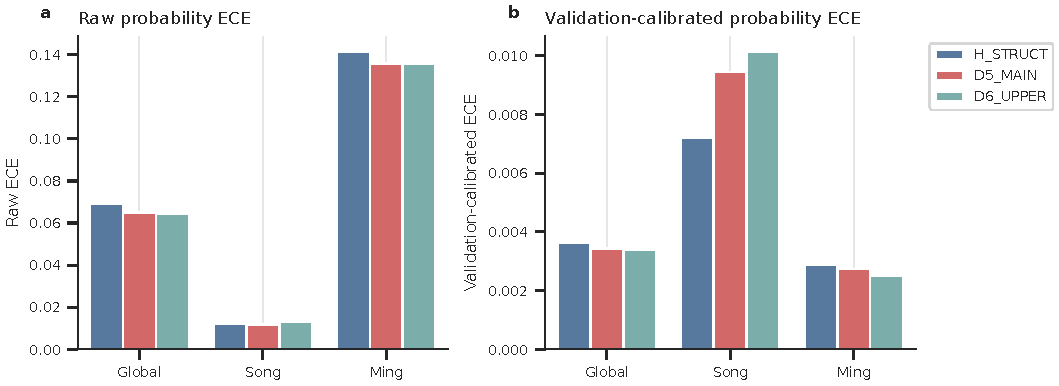
\includegraphics[width=0.84\textwidth]{figures/figA1_calibration.pdf}
\caption{\textbf{Raw and validation-calibrated ECE.} The sigmoid calibrator was fitted on validation predictions only. Lower ECE is better; the panels use different y-axis scales.}
\Description{Two grouped bar plots compare raw and validation-calibrated expected calibration error.}
\label{fig:calibration}
\end{figure}

\begin{figure}[!htbp]
\centering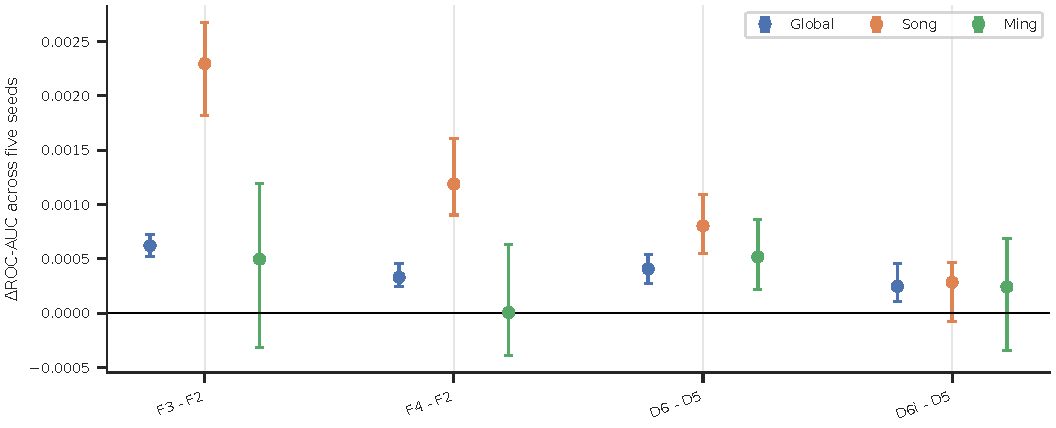
\includegraphics[width=0.84\textwidth]{figures/figA2_multiseed.pdf}
\caption{\textbf{Five-seed stability.} Points are mean incremental ROC-AUC values and whiskers span the observed minimum to maximum across five prespecified seeds.}
\Description{Points and error bars show four feature-block contrasts for Global, Song, and Ming.}
\label{fig:multiseed}
\end{figure}

\begin{figure}[!htbp]
\centering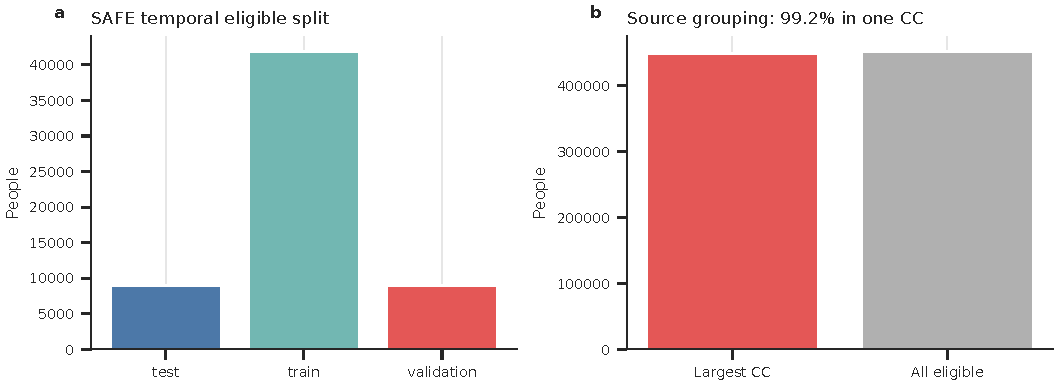
\includegraphics[width=0.84\textwidth]{figures/figA3_robustness_scope.pdf}
\caption{\textbf{Scope of uncompleted robustness tests.} \textbf{a}, Eligible people in the frozen SAFE temporal split, for which no locked performance artifact exists. \textbf{b}, The largest primary-source connected component compared with all eligible people.}
\Description{Bars show temporal split sizes and dominance of the largest source connected component.}
\label{fig:scope}
\end{figure}

\section{Complete Evaluation Notes}
Family holdout keeps connected family groups disjoint. Matched spatial comparisons restrict random and spatial tests to identical reliable-prefecture support, although the individuals differ. The SAFE temporal split uses whole years, with training through 1729, validation through 1821, and testing thereafter; 601,273 people are ineligible. Qing results remain descriptive because no frozen Qing holdout exists.

Calibration uses a validation-fitted sigmoid and ten ECE bins. Paired bootstrap intervals use 500 stratified resamples only where exact paired predictions were retained. Grouped SHAP uses 10,000-person samples for each of nine population-model combinations, and all additivity checks pass. The review bundle contains revised grouped, feature-level, and direction summaries with \texttt{historical\allowbreak\_regime} as the canonical dynasty group.

\FloatBarrier
\section{Frozen Parameters and Full Results}
\begin{longtable}{ll}
\caption{Frozen CatBoost and evaluation parameters. Validation chooses early stopping, class weighting, and thresholds; the test does not.}\label{tab:app-parameters}\\
\toprule
Parameter & Frozen value \\
\midrule
\endfirsthead
\toprule
Parameter & Frozen value \\
\midrule
\endhead
canonical\_seed & 42 \\
iterations & 500 \\
learning\_rate & 0.05 \\
depth & 7 \\
loss\_function & Logloss \\
eval\_metric & AUC \\
l2\_leaf\_reg & 5 \\
early\_stopping\_rounds & 80 \\
class\_weight\_candidates & ['None', 'Balanced'] \\
bootstrap\_resamples & 500 \\
calibration\_bins & 10 \\
\bottomrule
\end{longtable}

\begingroup
\renewcommand{\thetable}{A1b}
\renewcommand{\theHtable}{A1b}
\begingroup
\setlength{\tabcolsep}{4pt}
\begin{longtable}{>{\raggedright\arraybackslash}p{1.55cm}>{\raggedright\arraybackslash}p{1.75cm}>{\raggedright\arraybackslash}p{3.30cm}>{\raggedright\arraybackslash}p{1.45cm}>{\raggedright\arraybackslash}p{4.00cm}>{\raggedright\arraybackslash}p{3.90cm}}
\caption{Retained operating points for the frozen primary models. Numeric class weights were not serialized; the retained weighting scheme is reported without reconstruction. The sigmoid is $\sigma(a\,\mathrm{logit}(p)+b)$ and was fitted only on validation predictions.}\label{tab:app-operating}\\
\toprule
Population & Model & Selected weighting & Threshold & Objective / selection & Calibrator parameters \\
\midrule
\endfirsthead
\toprule
Population & Model & Selected weighting & Threshold & Objective / selection & Calibrator parameters \\
\midrule
\endhead
Global & Logistic M6 & balanced (logistic); numeric weights NOT\_RETAINED & 0.53 & binary logistic loss; lbfgs; frozen linear baseline & NOT\_RETAINED \\
Global & H\_STRUCT & Balanced (CatBoost); numeric weights NOT\_RETAINED & 0.47 & CatBoost Logloss; validation ROC-AUC, then lower LogLoss & $a=1.014113$; $b=-0.695780$ \\
Global & D5\_MAIN & Balanced (CatBoost); numeric weights NOT\_RETAINED & 0.53 & CatBoost Logloss; validation ROC-AUC, then lower LogLoss & $a=1.023418$; $b=-0.704666$ \\
Global & D6\_UPPER & Balanced (CatBoost); numeric weights NOT\_RETAINED & 0.49 & CatBoost Logloss; validation ROC-AUC, then lower LogLoss & $a=1.022593$; $b=-0.704377$ \\
Song & Logistic M6 & balanced (logistic); numeric weights NOT\_RETAINED & 0.53 & binary logistic loss; lbfgs; frozen linear baseline & NOT\_RETAINED \\
Song & H\_STRUCT & Balanced (CatBoost); numeric weights NOT\_RETAINED & 0.56 & CatBoost Logloss; validation ROC-AUC, then lower LogLoss & $a=0.996209$; $b=-0.079308$ \\
Song & D5\_MAIN & Balanced (CatBoost); numeric weights NOT\_RETAINED & 0.52 & CatBoost Logloss; validation ROC-AUC, then lower LogLoss & $a=0.996765$; $b=-0.103745$ \\
Song & D6\_UPPER & Balanced (CatBoost); numeric weights NOT\_RETAINED & 0.56 & CatBoost Logloss; validation ROC-AUC, then lower LogLoss & $a=1.008454$; $b=-0.099204$ \\
Ming & Logistic M6 & balanced (logistic); numeric weights NOT\_RETAINED & 0.49 & binary logistic loss; lbfgs; frozen linear baseline & NOT\_RETAINED \\
Ming & H\_STRUCT & Balanced (CatBoost); numeric weights NOT\_RETAINED & 0.52 & CatBoost Logloss; validation ROC-AUC, then lower LogLoss & $a=1.028157$; $b=-1.377243$ \\
Ming & D5\_MAIN & Balanced (CatBoost); numeric weights NOT\_RETAINED & 0.50 & CatBoost Logloss; validation ROC-AUC, then lower LogLoss & $a=1.049390$; $b=-1.359069$ \\
Ming & D6\_UPPER & Balanced (CatBoost); numeric weights NOT\_RETAINED & 0.47 & CatBoost Logloss; validation ROC-AUC, then lower LogLoss & $a=1.052307$; $b=-1.359874$ \\
\bottomrule
\end{longtable}
\endgroup

\endgroup
\setcounter{table}{1}
\begin{longtable}{llrrrrrrrr}
\caption{Full-precision locked primary-test metrics. Prevalence accompanies PR-AUC; ECE follows validation-fitted sigmoid calibration.}\label{tab:app-metrics}\\
\toprule
Population & Model & Prev. & ROC & PR & Bal. Acc. & F1 & LogLoss & Brier & ECE \\
\midrule
\endfirsthead
\toprule
Population & Model & Prev. & ROC & PR & Bal. Acc. & F1 & LogLoss & Brier & ECE \\
\midrule
\endhead
Global & Logistic M6 & 0.3339 & 0.916038 & 0.843596 & 0.848544 & 0.792425 & 0.363532 & 0.112821 & -- \\
Global & H\_STRUCT & 0.3339 & 0.926721 & 0.858211 & 0.860891 & 0.809549 & 0.339298 & 0.104816 & 0.003644 \\
Global & D5\_MAIN & 0.3339 & 0.936956 & 0.882535 & 0.869045 & 0.820769 & 0.315106 & 0.097356 & 0.003438 \\
Global & D6\_UPPER & 0.3339 & 0.937421 & 0.883128 & 0.869739 & 0.821732 & 0.313950 & 0.096938 & 0.003398 \\
Song & Logistic M6 & 0.4827 & 0.900769 & 0.880995 & 0.833327 & 0.831659 & 0.398458 & 0.122321 & -- \\
Song & H\_STRUCT & 0.4827 & 0.918350 & 0.911650 & 0.847816 & 0.842489 & 0.360396 & 0.111199 & 0.007191 \\
Song & D5\_MAIN & 0.4827 & 0.938351 & 0.939838 & 0.870885 & 0.865457 & 0.308890 & 0.093986 & 0.009439 \\
Song & D6\_UPPER & 0.4827 & 0.939798 & 0.941195 & 0.871448 & 0.866054 & 0.305452 & 0.092799 & 0.010154 \\
Ming & Logistic M6 & 0.1993 & 0.902058 & 0.776510 & 0.801988 & 0.696932 & 0.349956 & 0.112626 & -- \\
Ming & H\_STRUCT & 0.1993 & 0.910657 & 0.779909 & 0.813006 & 0.712249 & 0.346308 & 0.109660 & 0.002878 \\
Ming & D5\_MAIN & 0.1993 & 0.916395 & 0.800527 & 0.816932 & 0.726957 & 0.322947 & 0.102572 & 0.002736 \\
Ming & D6\_UPPER & 0.1993 & 0.916696 & 0.801196 & 0.817768 & 0.727861 & 0.322401 & 0.102311 & 0.002513 \\
\bottomrule
\end{longtable}

\begin{longtable}{lllrlll}
\caption{All grouped ablation contrasts. Intervals are shown only where the exact paired predictions were retained.}\label{tab:app-ablation}\\
\toprule
Population & Block & Contrast & $\Delta$ROC & ROC CI & $\Delta$PR & PR CI \\
\midrule
\endfirsthead
\toprule
Population & Block & Contrast & $\Delta$ROC & ROC CI & $\Delta$PR & PR CI \\
\midrule
\endhead
Global & Personal: gender & P1 - P0 & +0.052609 & -- & +0.057951 & -- \\
Song & Personal: gender & P1 - P0 & +0.047146 & -- & +0.024770 & -- \\
Ming & Personal: gender & P1 - P0 & +0.112030 & -- & +0.043581 & -- \\
Global & Address observability & A1 - A0 & +0.046510 & -- & +0.093855 & -- \\
Song & Address observability & A1 - A0 & +0.200425 & -- & +0.147162 & -- \\
Ming & Address observability & A1 - A0 & +0.054365 & -- & +0.047488 & -- \\
Global & Administrative geography & A2 - A1 & +0.018820 & -- & +0.076062 & -- \\
Song & Administrative geography & A2 - A1 & +0.102003 & -- & +0.166421 & -- \\
Ming & Administrative geography & A2 - A1 & +0.016509 & -- & +0.090486 & -- \\
Global & Physical geography & A3 - A2 & +0.000014 & -- & -0.000343 & -- \\
Song & Physical geography & A3 - A2 & +0.000311 & -- & +0.000883 & -- \\
Ming & Physical geography & A3 - A2 & +0.000152 & -- & +0.002470 & -- \\
Global & Address-record semantics & A4 - A3 & +0.008980 & -- & +0.022396 & -- \\
Song & Address-record semantics & A4 - A3 & +0.000514 & -- & +0.001088 & -- \\
Ming & Address-record semantics & A4 - A3 & +0.030118 & -- & +0.099341 & -- \\
Global & Family observability & F1 - F0 & +0.021728 & -- & +0.035438 & -- \\
Song & Family observability & F1 - F0 & +0.036438 & -- & +0.056570 & -- \\
Ming & Family observability & F1 - F0 & +0.088076 & -- & +0.105958 & -- \\
Global & Family topology & F2 - F1 & +0.002251 & [0.0019,0.0026] & +0.002381 & [0.0018,0.0029] \\
Song & Family topology & F2 - F1 & +0.009136 & [0.0074,0.0106] & +0.007811 & [0.0060,0.0095] \\
Ming & Family topology & F2 - F1 & +0.007871 & [0.0064,0.0094] & +0.010709 & [0.0087,0.0128] \\
Global & Family capital (full record) & F3 - F2 & +0.000701 & [0.0005,0.0009] & +0.001098 & [0.0007,0.0015] \\
Song & Family capital (full record) & F3 - F2 & +0.001821 & [0.0009,0.0027] & +0.001877 & [0.0006,0.0031] \\
Ming & Family capital (full record) & F3 - F2 & -0.000319 & [-0.0009,0.0002] & +0.000576 & [-0.0004,0.0015] \\
Global & Family capital (train observed) & F4 - F2 & +0.000311 & [0.0001,0.0005] & +0.000541 & [0.0002,0.0009] \\
Song & Family capital (train observed) & F4 - F2 & +0.000902 & [0.0002,0.0016] & +0.001049 & [0.0002,0.0019] \\
Ming & Family capital (train observed) & F4 - F2 & -0.000394 & [-0.0010,0.0002] & +0.000525 & [-0.0004,0.0014] \\
\bottomrule
\end{longtable}

\begingroup
\setlength{\tabcolsep}{3pt}
\begin{longtable}{>{\raggedright\arraybackslash}p{1.60cm}>{\raggedright\arraybackslash}p{2.00cm}>{\raggedright\arraybackslash}p{2.60cm}>{\centering\arraybackslash}p{1.45cm}>{\centering\arraybackslash}p{1.45cm}>{\centering\arraybackslash}p{1.45cm}>{\centering\arraybackslash}p{1.45cm}>{\raggedright\arraybackslash}p{3.60cm}}
\caption{Complete distribution-shift evidence. Dashes preserve experiments that were unavailable or infeasible rather than inventing estimates.}\label{tab:app-robustness}\\
\toprule
Population & Model & Protocol & Shift ROC & $\Delta$ROC & Shift PR & $\Delta$PR & Status \\
\midrule
\endfirsthead
\toprule
Population & Model & Protocol & Shift ROC & $\Delta$ROC & Shift PR & $\Delta$PR & Status \\
\midrule
\endhead
Global & D5\_MAIN & Matched-support spatial & 0.897571 & -0.022177 & 0.879052 & -0.035853 & RUN \\
Global & H\_STRUCT & Matched-support spatial & 0.872439 & -0.030714 & 0.831291 & -0.060427 & RUN \\
Song & D5\_MAIN & Matched-support spatial & 0.893811 & -0.024455 & 0.933361 & -0.026770 & RUN \\
Song & H\_STRUCT & Matched-support spatial & 0.810654 & -0.062065 & 0.852220 & -0.077701 & RUN \\
Ming & D5\_MAIN & Matched-support spatial & 0.932692 & -0.006423 & 0.920740 & -0.005574 & RUN \\
Ming & H\_STRUCT & Matched-support spatial & 0.922810 & -0.007297 & 0.895060 & -0.010600 & RUN \\
Global & F2 structural comparator & Family-group holdout & 0.927159 & -0.002154 & 0.866816 & -0.001824 & RUN \\
Ming & F2 structural comparator & Family-group holdout & 0.908970 & -0.003194 & 0.789235 & -0.003727 & RUN \\
Global & Locked models & SAFE temporal & -- & -- & -- & -- & SPLIT\_\allowbreak ONLY\_\allowbreak NO\_\allowbreak LOCKED\_\allowbreak PERFORMANCE \\
Qing & Locked models & Qing dynasty holdout & -- & -- & -- & -- & NOT\_\allowbreak RUN\_\allowbreak NO\_\allowbreak FROZEN\_\allowbreak HOLDOUT \\
Global & H\_\allowbreak STRUCT/\allowbreak D5\_\allowbreak MAIN & Source group & -- & -- & -- & -- & SOURCE\_\allowbreak GROUP\_\allowbreak CONFIRMATION\_\allowbreak NOT\_\allowbreak FEASIBLE \\
\bottomrule
\end{longtable}
\endgroup


\section{Complete Frozen Feature Registry}
\begin{longtable}{lll}
\caption{Complete frozen feature registry. Repeated features document the exact membership of each locked model.}\label{tab:app-features}\\
\toprule
Model & Feature & Role \\
\midrule
\endfirsthead
\toprule
Model & Feature & Role \\
\midrule
\endhead
H\_STRUCT & dynasty\_name & categorical \\
H\_STRUCT & gender & categorical \\
H\_STRUCT & safe\_birth\_decade & categorical \\
H\_STRUCT & province\_id & categorical \\
H\_STRUCT & prefecture\_id & categorical \\
H\_STRUCT & county\_id & categorical \\
H\_STRUCT & has\_safe\_birth\_year & numeric \\
H\_STRUCT & has\_geography & numeric \\
H\_STRUCT & has\_valid\_coordinates & numeric \\
H\_STRUCT & latitude & numeric \\
H\_STRUCT & longitude & numeric \\
H\_STRUCT & distance\_to\_dynasty\_capital\_km & numeric \\
H\_STRUCT & train\_region\_person\_count & numeric \\
H\_STRUCT & train\_region\_log\_density & numeric \\
H\_STRUCT & has\_kin & numeric \\
H\_STRUCT & has\_core\_family & numeric \\
H\_STRUCT & father\_identified & numeric \\
H\_STRUCT & mother\_identified & numeric \\
H\_STRUCT & any\_grandfather\_identified & numeric \\
H\_STRUCT & n\_known\_parents & numeric \\
H\_STRUCT & n\_known\_grandparents & numeric \\
H\_STRUCT & n\_known\_ancestors & numeric \\
H\_STRUCT & n\_known\_same\_generation & numeric \\
H\_STRUCT & n\_known\_descendants & numeric \\
H\_STRUCT & n\_known\_core\_kin & numeric \\
H\_STRUCT & family\_group\_size & numeric \\
D5\_MAIN & dynasty\_name & categorical \\
D5\_MAIN & gender & categorical \\
D5\_MAIN & safe\_birth\_decade & categorical \\
D5\_MAIN & province\_id & categorical \\
D5\_MAIN & prefecture\_id & categorical \\
D5\_MAIN & county\_id & categorical \\
D5\_MAIN & addr\_type\_name & categorical \\
D5\_MAIN & has\_address & numeric \\
D5\_MAIN & has\_kin & numeric \\
D5\_MAIN & has\_assoc & numeric \\
D5\_MAIN & has\_status & numeric \\
D5\_MAIN & has\_text & numeric \\
D5\_MAIN & has\_institution & numeric \\
D5\_MAIN & documentation\_intensity & numeric \\
D5\_MAIN & has\_safe\_birth\_year & numeric \\
D5\_MAIN & has\_geography & numeric \\
D5\_MAIN & has\_valid\_coordinates & numeric \\
D5\_MAIN & latitude & numeric \\
D5\_MAIN & longitude & numeric \\
D5\_MAIN & distance\_to\_dynasty\_capital\_km & numeric \\
D5\_MAIN & train\_region\_person\_count & numeric \\
D5\_MAIN & train\_region\_log\_density & numeric \\
D5\_MAIN & local\_target\_prior & numeric \\
D5\_MAIN & has\_core\_family & numeric \\
D5\_MAIN & father\_identified & numeric \\
D5\_MAIN & mother\_identified & numeric \\
D5\_MAIN & any\_grandfather\_identified & numeric \\
D5\_MAIN & n\_known\_parents & numeric \\
D5\_MAIN & n\_known\_grandparents & numeric \\
D5\_MAIN & n\_known\_ancestors & numeric \\
D5\_MAIN & n\_known\_same\_generation & numeric \\
D5\_MAIN & n\_known\_descendants & numeric \\
D5\_MAIN & n\_known\_core\_kin & numeric \\
D5\_MAIN & family\_group\_size & numeric \\
D6\_UPPER & dynasty\_name & categorical \\
D6\_UPPER & gender & categorical \\
D6\_UPPER & safe\_birth\_decade & categorical \\
D6\_UPPER & province\_id & categorical \\
D6\_UPPER & prefecture\_id & categorical \\
D6\_UPPER & county\_id & categorical \\
D6\_UPPER & addr\_type\_name & categorical \\
D6\_UPPER & has\_address & numeric \\
D6\_UPPER & has\_kin & numeric \\
D6\_UPPER & has\_assoc & numeric \\
D6\_UPPER & has\_status & numeric \\
D6\_UPPER & has\_text & numeric \\
D6\_UPPER & has\_institution & numeric \\
D6\_UPPER & documentation\_intensity & numeric \\
D6\_UPPER & has\_safe\_birth\_year & numeric \\
D6\_UPPER & has\_geography & numeric \\
D6\_UPPER & has\_valid\_coordinates & numeric \\
D6\_UPPER & latitude & numeric \\
D6\_UPPER & longitude & numeric \\
D6\_UPPER & distance\_to\_dynasty\_capital\_km & numeric \\
D6\_UPPER & train\_region\_person\_count & numeric \\
D6\_UPPER & train\_region\_log\_density & numeric \\
D6\_UPPER & local\_target\_prior & numeric \\
D6\_UPPER & has\_core\_family & numeric \\
D6\_UPPER & father\_identified & numeric \\
D6\_UPPER & mother\_identified & numeric \\
D6\_UPPER & any\_grandfather\_identified & numeric \\
D6\_UPPER & n\_known\_parents & numeric \\
D6\_UPPER & n\_known\_grandparents & numeric \\
D6\_UPPER & n\_known\_ancestors & numeric \\
D6\_UPPER & n\_known\_same\_generation & numeric \\
D6\_UPPER & n\_known\_descendants & numeric \\
D6\_UPPER & n\_known\_core\_kin & numeric \\
D6\_UPPER & family\_group\_size & numeric \\
D6\_UPPER & father\_ever\_entry & numeric \\
D6\_UPPER & father\_ever\_posting & numeric \\
D6\_UPPER & paternal\_grandfather\_ever\_entry & numeric \\
D6\_UPPER & paternal\_grandfather\_ever\_posting & numeric \\
D6\_UPPER & maternal\_grandfather\_ever\_entry & numeric \\
D6\_UPPER & maternal\_grandfather\_ever\_posting & numeric \\
D6\_UPPER & n\_older\_kin\_ever\_entry & numeric \\
D6\_UPPER & n\_older\_kin\_ever\_posting & numeric \\
D6\_UPPER & older\_kin\_entry\_ratio & numeric \\
D6\_UPPER & older\_kin\_posting\_ratio & numeric \\
\bottomrule
\end{longtable}


\section{Reproduction Command}
From the project root, run \texttt{bash scripts/run\_phase3\_1\_1\_final\_polish.sh}. The runner verifies the Phase 3.1 baseline, rebuilds only Phase 3.1.1 tables and figures, compiles both manuscripts, renders every PDF page, runs audits and tests, packages the deliverables, and validates both archives.
\label{appendixend}

\end{document}
